\cotefile{29}
\scanpage{77}
\mspage{\unsure{L|2|7}}

pour les modèles normaux (\unsure{résultant} de la partie facile de Lefschetz, en \unsure{vers.|version} pour les groupes fondamentaux rendus abéliens), on a fini. De façon plus précise il suffit, prenant un \inserted{modèle} $X$ \uline{projectif} sur $k$, (propre et normal), de prendre dans $X$ une ``courbe générique $C$'' et pour $\unsure{n|u}(K)$ le genre de la dite courbe générique.

% diagram in left margin, opposite the last two lines
\diagram{\begin{tikzcd}[ampersand replacement=\&,column sep=0.4em,row sep=1.1em]
 C' \arrow[d] \& {\subset} \& X' \arrow[d] \& \& \\
 C_{\unsure{k(u)|K(u)}} \& {\subset} \& X \& {\subset} \& P^{r}
\end{tikzcd}}

Y-a-t-il une démonstration du fait que cela donne une majoration, n'utilisant pas la théorie du groupe fondamental et le fait que $\underline{\mathrm{Pic}}^{\tau}_{X/k}$ est propre sur $k$ si $X$ est normale ?
% slanted
\margin{démonstration directe ???}
% archive sheet number: 76
\scanpage{78}

\deleted{\unsure{Comparaison|Comportement} d'un anneau hensélien et son complété ($\pi_1$, \unsure{descente|discret} etc\unsure{...|.|. \ldots})}

\uline{Revêtements formels} \uline{étales} \uline{et th. de Mumford}
% archive sheet number: 77
\scanpage{82}
% Mirrored typescript shows through from the reverse.
\diagram{\begin{tikzcd}[ampersand replacement=\&,column sep=.7em,row sep=.1em]
 \mathrm{I} \& 3 \& \& \\
 \& 7 \arrow[dr,dash] \& \& \text{restrict to adic morphisms}\\
 \& \& 9 \& \\
 \& 11 \arrow[ur,dash] \& \& \\
 \& 12 \& \&
\end{tikzcd}}
\margin{ambiguity on point of formal schemes quite general \unsure{---}}

\deleted{18 --- Most examples come from usual \unsure{qu. pr.|pr.|gp.} schemes over $\mathbb Z$\unsure{!|/}}

20

27

whole chapter looks \unsure{plethoric}

\diagram{\begin{tikzcd}[ampersand replacement=\&,column sep=.5em,row sep=.45em]
 {} \& {} \& |[draw,rounded corners]|{\parbox{.44\linewidth}{\unsure{repetitio|topological} interpretation of $\pi_1^D$ in terms of $S-\operatorname{Supp}D$}} \arrow[dddl,leftrightarrow] \\
 {\mathrm{II}} \& {\begin{gathered}2\\12\ \text{unreasonable !}\\16\\20\\22\end{gathered}} \& |[draw]|{\parbox{.44\linewidth}{Copy of previous note on tame ramification ?}}\\
 {} \& {} \& |[draw]|{\parbox{.44\linewidth}{Include variant of Lefschetz's Theorem for $\pi_1^t$}}\\
 {} \& |[draw,rounded corners]|{\parbox{.23\linewidth}{whole chapter $\overline{\mathrm{III}}$ seems to be used only to get \fbox{3.5.8}}} \& |[draw]|{\parbox{.44\linewidth}{Include, after Mumford's Theorem, application to question of finite generation of local \deleted{tame} \inserted{prime to $p$} fund. group.}}
\end{tikzcd}}

$\mathrm{III}$ \uline{1}

2

6 \quad 2 fois

8

11

$12^{b}$

16 \quad add section on case when $D\unsure{{}_i|{}}$'s have equations ! This should make the situation much clearer ! For instance 3.4.1, 3.4.2

22

25 \quad fpqc descent for tamely ramified coverings ? At least one would like to have a ``champ'' on $\mathrm{Et}_{/S}$ !

\diagram{\begin{tikzcd}[ampersand replacement=\&,column sep=.65em,row sep=.35em]
26 \& \left\{\begin{gathered}\text{a)}\\\text{b)}\end{gathered}\right. \& \text{Normality assumption over integral (formal normality}\\
28 \& 15 \& \text{in base formal schemes\unsure{...})}\\
{} \& {\text{cf 3.6.6}} \arrow[uul,dash,bend left] \& {}
\end{tikzcd}}

Proof of 3.6.5 is \unsure{unbelievedly|unbelievably} long !

\fbox{where is the ``Abhyankar lemma\unsure{.|{}}'' ?}
% archive sheet number: 81
\scanpage{84}
% Mirrored typescript shows through from the reverse.
$\underline{\overline{\mathrm{IV}}}$ \quad \unsure{4.1.2|\S1\textsuperscript{2}} \qquad 4.1.2 \quad \unsure{treat|drawn} in terms of $\mathrm{III}$ p. 16. added.

Rather \inserted{\unsure{for $s^{*}$}} cumbersome\unsure{;|,} take point of $\operatorname{Spec}(\mathcal O_{S,s})$ !

6 \qquad Introduce geometric points of $S$.

% margin note written sideways
\margin{not needed ?!}
$\underline{\overline{\mathrm{VI}}}$ \quad 2 \quad \unsure{trivial|twice}

7 \quad What is the meaning ?

$\left.\begin{gathered}9\\11\end{gathered}\right\}$ \quad 6.1.1 and 6.2.2. could be made into a single example !

$\curvearrowleft\ \mathrm{VII}$ \quad 1

\margin{to check !}2 \quad I guess that one has \unsure{equivalence|equivalences} of categories anyhow !!

9

$\underline{\overline{\mathrm{VIII}}}$ \quad 1

2

3/8.1.6 Not too clear. Say that if
\deleted{$A$ a local or} \deleted{a local}
\inserted{$S$ any scheme}
\deleted{henselian ring, then to any}
(for instance the localization of $S$ at $s_0$) and
\deleted{$s_0,s_0^{*}$ two points,}
$x,y$ \unsure{to|two} points, $x\in\overline{\{y\}}$,
\deleted{then the} with geom point given, $\bar x,\bar y$,
$\overline{k(x)}/k,\ \overline{k(y)}/y$, then the ``paths'' \inserted{$\unsure{p}$}/ of $\bar y$ to $\bar x$
\deleted{$\unsure{\bar x\text{ to }\bar y|\bar x\otimes\bar y}$}
correspond exactly to the \deleted{point} liftings

\diagram{\begin{tikzcd}[ampersand replacement=\&,column sep=1.3em,row sep=.8em]
 {\bar S=\substack{\text{strict loc.}\\\text{of } S\text{ at }\bar x}}\arrow[d] \& \bar y^{\unsure{*|'|{}}}\arrow[l,dashed]\arrow[dl]\\
 S\&{}
\end{tikzcd}}

i.e. to the \inserted{$k(y)$-}hom of
\[
 \operatorname{ring}(\bar S\otimes_S y)=\prod K_i
 \ \text{into }\overline{k(y)}.
\]

$\underline{\overline{\mathrm{IX}}}$ \quad \uline{1} \qquad 14 \deleted{\unsure{de|do|etc.}}\qquad $9.3.4\Rightarrow9.3.5$ looks tautological

4 \qquad $9.3.5\Rightarrow9.3.2$ very cumbersome !

% slanted
\margin{yoga stemming from Abhyankar lemma to be used\unsure{...|{}}}
$5,6$

9

$10'$ \qquad 18

$10''$ \qquad 19

12
% archive sheet number: 83
\scanpage{85}
\mspage{\handwritten{69}}\mspage{\handwritten{1}}

% A single diagonal stroke runs through the whole typescript.
\deleted{Appliquons \deleted{\unsure{(1|1.|1}}{\handwritten{7}}.2.1\deleted{\unsure{)|à}} au groupe formel $\handwritten{\hat}{A}$, dans le cas favorable envisagé dans \deleted{\unsure{le|7.0|la}} 7.1 où le schéma \deleted{\unsure{abél|Abél|ab.}} formel abélien $\handwritten{\hat}{B}$ est algébrisable\handwritten{,} \inserted{\handwritten{et où on suppose de plus \deleted{\unsure{le}} $T_0$ isotrivial.}} On trouve alors un\deleted{e extension canonique du} schéma \deleted{abélien $B$ dont le}\inserted{\handwritten{en groupes $A^{\unsure{\natural|\sharp}}$ sur $S$}}, \inserted{\handwritten{appelé le \uline{groupe de Raynaud} associé au schéma en groupes $A$ sur $S$\unsure{,|$\vphantom{S}_{o}$,} tel que $A$}} complété formel est $B$, par le tore $T$ sur $S$ qui remonte $T_0$\handwritten{,}\deleted{\unsure{;|,|et}} que nous ap\handwritten{p}ellerons l'\uline{extension de Raynaud} associée à $A$, et que nous noterons $A^{\handwritten{\natural}}$ :
\[
 0\handwritten{\longrightarrow}T\handwritten{\longrightarrow}A^{\handwritten{\natural}}\handwritten{\longrightarrow}B\handwritten{\longrightarrow}0\ .
 \tag*{(\deleted{1}\handwritten{7}.2.2)}
\]
Elle est donc définie, à isomorphisme unique près, par le fait qu'elle donne naissance à un système cohérent d'isomorphismes d'extensions
\[
 A^{\handwritten{\natural}}_n\handwritten{\simeq}A_n
 \tag*{(7.2.\handwritten{3})}
\]
(le deuxième membre muni de sa structure d'extension décrite dans (7.1.1) i.e. qu'on a un isomorphisme de \inserted{schémas formels en} groupes \deleted{formels}
\[
 (A^{\handwritten{\natural}})^{\handwritten{\wedge}}\handwritten{\simeq}\handwritten{\hat}{A}\ ,
 \tag*{(7.\deleted{3}\handwritten{2}.4)}
\]
respectant d'ailleurs les structures d'extensions. \deleted{Il résulte de plus de 7.2.1}

7.2.5. Il résulte d'autre part \deleted{que la} immédiatement de 7.2.1 que la suite exacte (7.2.2) dépend fonctoriellement du schéma \inserted{en groupes} $A$ sur $S$ satisfaisant aux conditions envisagées dans 7.1, et que sa formation commute à tout changement de base par un homomorphisme $S'\handwritten{\to} S$ associé à un homomorphisme d'anneaux topologiques noethériens adiques $V\handwritten{\to}V'$.}
% archive sheet number: 84
\scanpage{86}

$\mathrm{X}$ \quad 1 \qquad \unsure{extends|exists|works} (and is useful) in quasi coherent case. State that $\mathcal E$ is of finite type (resp. finite presentation) \inserted{\unsure{i.e.|etc.|or} loc free} iff $\unsure{\mathcal E_1|\varepsilon_1},\mathcal E_2$ are.

\unsure{d}

\margin{$\times$}5 \hfill $+S_3$

12 \qquad Amounts to showing : $\unsure{\mathscr X|X}$ finite flat covering of $S$ is tame with r. to $D_1,D_2$ iff it \deleted{\unsure{is so}} restriction to $S_1,S_2$ are tamely ramified

\uline{Should be trivial} with the conditions considered !
% archive sheet number: 85
\scanpage{87}

% One long cancellation stroke crosses both blocks.
\deleted{Voyons alors la notion \uline{d'image inverse des $O$-Modules}. Un $O$-Module quasi-cohérent est transformé en idem, donc \uline{Module} \inserted{\unsure{qu. coh.|quasi-coh.|fini cohérent}} \uline{stratifié} est transformé en idem. Il faut vérifier que c'est la notion \unsure{intuitive} d'image inverse des Modules stratifiés.

\medskip\centerline{\rule{2em}{.4pt}}\medskip

Supposons que \deleted{\unsure{Si|si}} $X'\unsure{-|\to} X\times_S S'$ soit une \unsure{imm} (plus gén \deleted{\unsure{un}} non ramifié) alors le morphisme $T_0\times_X X'-T\times_S S'$ est \unsure{égalt} une imm (resp. non ramifié) et peut être muni de la famille des voisinages infinitésimaux de tous ordres,

\diagram{\begin{tikzcd}[ampersand replacement=\&,column sep=.5em,row sep=.4em]
 {} \& T_0\arrow[dl]\arrow[ddd,hook] \& {} \& {} \& {}\\
 X\arrow[ddd] \& {} \& {} \& T_0\times_S S'\arrow[ull]\arrow[dl,dash]\arrow[ddd,hook] \& {}\\
 {} \& {} \& X\times_S S'\arrow[ull]\arrow[ddd] \& {} \& {T_0\times_X X'=T'_0}\arrow[ul,"\mathrm{n.r}"]\arrow[dl]\arrow[ddl,dashed,"\mathrm{n.r.}"]\\
 {} \& T\arrow[dl] \& {} \& X'\arrow[ul,"\mathrm{n.r.}"']\arrow[d]\arrow[ddl,very thick] \& {}\\
 S \& {} \& {} \& T\times_S S'\arrow[ull]\arrow[dl,dash] \& {}\\
 {} \& {} \& S'\arrow[ull] \& {} \& T'\arrow[ul]
\end{tikzcd}}

(soit $T'_{\unsure{(n)|n}}$). Alors $f^{*}(\unsure{\mathscr F|\mathscr G|\mathcal F})=\varinjlim_n\mathscr F'_n$ (\unsure{bien|comme} \unsure{entendu|on a donné}) \unsure{si|où} $F'$ est un faisceau}
% archive sheet number: 86
\scanpage{88}
\mspage{1.}
% A reversed typescript is visible through the sheet.
$\unsure{\mathfrak X|\mathscr X|\mathcal X}$ schéma formel régulier, \inserted{connexe}, $\mathfrak X_0=X_0$ diviseur régulier, $D\deleted{\unsure{=}}=\bigcup_0^{\unsure{r|n}}D_i$ diviseur \deleted{avec} normal crossings \unsure{seulement|deux à deux} $D_0=X_0$, [les $D_i$ réguliers \unsure{individuellement|irréductibles}] . $D'=\sum_{i\ne0}D_i$, $D'_0$ induit sur $X_0$.

\figure{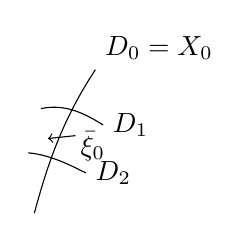
\begin{tikzpicture}[x=.52cm,y=.52cm]
\draw (-.65,-1.6) .. controls (-.3,-.3) and (.08,.75) .. (.84,1.9) node[above right] {$D_0=X_0$};
\draw (-.49,.95) .. controls (.11,1.08) and (.6,.82) .. (1.03,.55) node[right] {$D_1$};
\draw (-.8,-.13) .. controls (-.2,-.18) and (.37,-.51) .. (.61,-.62) node[right] {$D_2$};
\draw[->] (.35,.29)--(-.32,.22);
\node[right] at (.24,.03) {$\bar\xi_0$};
\end{tikzpicture}}

\diagram{\begin{tikzcd}[ampersand replacement=\&,column sep=.52em,row sep=.45em]
 e\arrow[r]\& I_0\arrow[r]\& \pi_1^t(\mathfrak X/D,\bar\xi_1)\arrow[r]\& \pi_1^t(X_0/D'_0,\bar\xi_0)\arrow[r]\&e\\
 {}\&{}\&\pi_1^t(\mathfrak X/D)\arrow[u,equal]\&\pi_1^t(U)\arrow[u,equal]\&\pi_1(\mathfrak X/D',\bar\xi_{\unsure{1|0}})\arrow[ul,equal]\\
 {}\&{}\&{}\&D_0-D'_0\arrow[u,equal]\&\Bigg\}
\end{tikzcd}}

\diagram{\begin{tikzcd}[ampersand replacement=\&,column sep=1.25em,row sep=.5em]
 \deleted{\unsure{\mu}}\arrow[r]\&\mu^\infty_{X_0,\mathrm{tame}}(\bar\xi_0)\arrow[r]\& I_0\arrow[r]\&0\\
 {}\&\mu(\deleted{\unsure{\bar\xi}})\arrow[u,equal]\&{}\&{}
\end{tikzcd}}
\margin{$=\varprojlim_{n>0}\mu_n$ \ $n$ inversible dans $\mathcal O_{X_0}$}

\diagram{\begin{tikzcd}[ampersand replacement=\&,column sep=1.2em,row sep=.3em]
 \mu\arrow[r]\& I\arrow[r]\&0\\
 \mu^\infty_{X_0,\mathrm{tame}}\arrow[u,equal]\&{}\&\text{faisceaux étale sur }X_0
\end{tikzcd}}

Donc
\[
 \prod_{\ell\,\unsure{\mathcal O_{X_0}=\mathcal O_{X_0}|\mathcal O_{X_0}^{*}|\ne p}}\mathbb Z_{\ell}
\]
\[
 \mu(\bar\xi_0)\longrightarrow\pi_1^t(\mathfrak X/D)\longrightarrow\pi_1^t(U)\longrightarrow e
\]

Opération de $\pi_1^t(U)$ sur $I_0$ via opérations de $\pi_1^{\unsure{t}}(U)$ sur $\deleted{\unsure{I}}\mu$ \deleted{\unsure{via opé|via opér.} ---}. Extension donnée par
\[
 \alpha\deleted{\unsure{\xi}}\in H^2(\pi_1^t(U),I_0)
 \qquad\qquad \deleted{\unsure{\xi}}\alpha=\,?
\]

% slanted
\margin{for all $H^i$, $i>0$, \uline{true} if $D_0$ \uline{is \uline{curve} over a} \uline{field}}
\uline{Lemme} 1. Soit $\widetilde U^t$ rev. étale de $U$ défini par $\pi_1^t$. Alors $H^1(\widetilde U^t,J\inserted{\text{constant}})=0$ si $\unsure{\#J|\mathcal J}$ premier aux car. résiduelles de $X_0$ [p. ex. $J=I$].

% slanted
\margin{Serre-Hochschild $H^{*}(U,J)\Leftarrow H^p(\pi_1^t,H^q(\widetilde U^t,\widetilde J))$}
\diagram{\begin{tikzcd}[ampersand replacement=\&,column sep=.55em,row sep=.35em]
0\arrow[r]\&H^2(\pi_1^t,I)\arrow[r,"\rho"]\& H^2(U,I)\arrow[r]\& H^2(\widetilde U^t,I_0\inserted{\text{constant sur }\widetilde U^t})^{\pi_1^t}\arrow[r]\& \bigl[H^3(\pi_1^t,I)\arrow[d]\\
{}\&{}\&{}\&\operatorname{Hom}(H_2(\widetilde U^t),I)^{\pi_1^t}\arrow[u,equal]\&\bigl.H^3(U,I)\bigr]\\
{}\&{}\&{}\&\operatorname{Hom}(\pi_2^t(U),I)^{\pi_1^t}\arrow[u,equal]\&{}
\end{tikzcd}}

\deleted{\unsure{f|$\rho$} \unsure{can.}} Donc $\alpha$ connu quand on connaît $\rho(\alpha)$, et l'image de \unsure{plus|$\rho(\alpha)$} dans $H^2(\widetilde U^t,I)^{\pi^t}\simeq\operatorname{Hom}(\pi_{2}^t(U),I)^{\pi_1^t}$ est nulle.
% archive sheet number: 87
\scanpage{89}
% Typescript read after a half turn.
Signalons pour finir ces généralités, que la formation des duals $D(G)$ commute à l'extension de la base, qui transforme donc groupes réflexifs en groupes réflexifs.

Nous nous intéressons par la suite au cas où $\underline C=(\mathrm{Sch})_{/S}$, catégorie des préschémas sur $S$, et $I=\underline G_{m\ S}$, le ``groupe multiplicatif sur $S$'', cf exposé I. Pour tout groupe \deleted{commutatif} ordinaire $M$, nous considérons le $S$-groupe $M_S$. On voit aussitôt que pour tout schéma en \unsure{groupes|groupe} $I$ sur $S$, on a un isomorphisme canonique (fonctoriel en $M,I$ et compatible avec l'extension de la base):
\[
 \operatorname{Hom}_{S\text{-gr}}(M_S,I)=\operatorname{Hom}_{\mathrm{gr}}(M,I\ (I/S))
\]
Appliquant ceci à un $S'$ variable sur $S$, on trouve un isomorphisme \inserted{fonctoriel}
\[
 D(M_S)(S')\qquad \operatorname{Hom}_{\mathrm{gr}}(M,\underline G_m(S'))
\]
On retrouve le foncteur déjà considéré dans l'exposé I, \inserted{aussi noté $D(M)$,} qui est représentable \deleted{\unsure{par} \unsure{comme}} pour $M$ commutatif comme
\[
 D(M)=D(M_S)=\operatorname{Spec}\ \underline O_S\ M
\]
où $\underline O_S\ M$ désigne l'Algèbre du groupe $M$ à coéfficients dans $\underline O_S$. (No\deleted{\unsure{On le}}tons \inserted{d'ailleurs dans le cas général} que $D(M)$ ne change pas si on remplace $M$ par $M$ rendu \deleted{\uline{Définition} 1.1. Un} abélien, de sorte \deleted{\unsure{qu'il n'y a pas d'inconv}} qu'on ne perd rien en supposant $M$ commutatif).

\uline{Définition} 1.1. Un schéma en groupes \inserted{$G$} sur $S$ est dit diagonalisable s'il est isomorphe à un schéma de la forme \deleted{\unsure{$D($}} $D(M)=D(M_S)=\underline{\operatorname{Hom}}_{S\text{-gr}}(M_S,\underline G_{\underline m}$ pour un groupe commutatif $M$ convenable. On dit que $G$ est localement diagonalisable, si tout point de $S$ admet un voisinage ouvert $U$, tel que $G\ U$ soit diagonalisable.

\deleted{\uline{Définition} 1.2. Un schéma en groupes $I$ sur $S$ est appelé un \uline{réseau constant} (resp. un réseau \uline{localement constant}) s'il est isomorphe à un schéma en}
% archive sheet number: 88
\scanpage{90}
\mspage{2.}
\margin{$i:X_0\to\unsure{\mathfrak X|\mathscr X|\mathcal X}$}

\uline{Lemme 2} Soit $\beta\in H^2(X_0,\underline\mu)$ la classe self-intersection de $X_0$ dans $\mathfrak X$, i.e. \inserted{la classe de \deleted{de} Chern \deleted{\unsure{et}} de} $\deleted{\unsure{\mathcal L}}T_{X_0/\mathfrak X})\simeq i^*(\underline L(X_0))$. Soit $\sigma:H^2(x,\mu)\unsure{-|\to}H^2(U,I)$ l'hom canonique. Alors
\[
 \rho(\alpha)=\sigma(\beta).
\]

Cela détermine l'\uline{extension} $\alpha$, sous réserve de connaître le quotient $I$ de $\mu$. On sait déjà que le \unsure{composé}
\diagram{\begin{tikzcd}[ampersand replacement=\&,column sep=.5em,row sep=.5em]
 {}\&H^2(\widetilde U^t,\widetilde\mu)\simeq\operatorname{Hom}(\pi_2^t(\unsure{X|U}),\mu_0)\&{}\&{}\\
 H^2(U,\mu)\arrow[r]\arrow[ur]\&H^2(U,I)\arrow[r]\&H^2(\widetilde U^t,I_0)=\operatorname{Hom}(\pi_2^t(U),I_0\&{}\\
 \deleted{\unsure{\rho(\beta)}}\quad\beta|U\arrow[u,equal]\&{}\&{}\&{}
\end{tikzcd}}
s'annule sur $\rho(\alpha)$. On a le diagramme (\unsure{comm.|commutatif}\inserted{par lemme 2}),
% slanted
\margin{Du moins si les $D'_i\subset X_0$ ($1\leq i\leq\unsure{n|r}$) sont \uline{disjoints} [à vérifier si cela est indispensable]}

\diagram{\begin{tikzcd}[ampersand replacement=\&,column sep=1em,row sep=1em]
 \pi_2^t(U)=H_2(\widetilde U)\arrow[d,"\overline\beta"]\arrow[dr,"\overline{\rho(\alpha)}"]\arrow[r,dash,"\deleted{\unsure{\longrightarrow}}"]\&\deleted{\pi_2^t(U)=H_2(\widetilde U^t)}\arrow[d,"\alpha","\deleted{\unsure{\rho}}"' ]\&{}\\
 \mu_0\arrow[r]\&\deleted{\unsure{\mu_0}}\unsure{I_0}\arrow[r,dash,"\deleted{\unsure{\longrightarrow}}"]\&\deleted{\unsure{I}}
\end{tikzcd}}
et par lemme 1. Ceci \unsure{bien} \unsure{---} défini l'hom. \deleted{dans} du $\pi_2^t$ défini par une 2-classe ].

Donc \deleted{\unsure{Im}} $\mu_0\to I_0$ s'\uline{annule} \uline{sur} $\operatorname{Im}\pi_2^t(U)$. Je dis que \deleted{\unsure{elle est}} le noyau
% slanted
\margin{\uline{\unsure{Heuristique}}}
est \uline{égal} à cette image ! [En fait, si $I'_0\ \unsure{\mathrm{de}|{}}=\deleted{\unsure{I}}\mu_{\unsure{\infty0|0}}/\operatorname{Im}\pi_2^t(U)$, on aura que $\operatorname{Im}\beta\in\operatorname{Ker}(H^2(U,I'_0)\unsure{-|\to}H^2(\widetilde U^t,I'_0))\simeq H^2(\pi_1^t,I'_0)$, donc $I\beta$ \uline{définit une extension}
% archive sheet number: 89
\scanpage{91}
% Typescript read after a half turn.
disjoints. \unsure{Donc|Dnnc} la donnée d'un homomorphisme de groupes $G\qquad\underline G_{m\ S}$ équivaut à la donnée d'une décomposition de $S$ comme réunion d'ouverts $S_m$ ($m\quad M$) deux à deux disjoints, i.e. à la donnée d'une application localement constante de $S$ dans $M$. Cela établit 1.3. donc 1.2.

\uline{Corollaire} 1.4. Un groupe diagonalisable est réflexif, donc aussi un groupe localement diagonalisable. Si $M,N$ sont deux groupes commutatifs ordinaires, \deleted{\unsure{on a}} l'homomorphisme naturel
\[
 \operatorname{Hom}_{S\text{-gr}}(M_S,N_S)\qquad\operatorname{Hom}_{S\text{-gr}}(D(N_S),D(M_S))
\]
est bijectif.

Notons maintenant que si $M$ est un groupe commutatif \uline{de type fini}, \deleted{\unsure{donc|fini}} donc défini par un nombre fini de générateurs et un nombre fini de relations, alors pour tout \deleted{préschéma en groupes $G$ sur $S$, on a une} \inserted{groupe ordinaire $N$,} l'application naturelle

On en déduit un isomorphisme de foncteurs sur $S$\unsure{:|=}
\[
 \underline{\operatorname{Hom}}_{S\text{-gr}}(M_S,N_S)\qquad\underline{\operatorname{Hom}}_{S\text{-gr}}(D(N_S),D(M_S))
\]
D'autre part \unsure{on|un} définit de façon évidente un homomorphisme
\[
 \operatorname{Hom}_{\mathrm{gr}}(M,N)_S\qquad\underline{\operatorname{Hom}}_{S\text{-gr}}(M_S,N_S)\ ,
\]
qui est toujours \deleted{\unsure{inj.}} un monomorphisme, et qui est un isomorphisme dès que $M$ est de type fini. On trouve ainsi:

\uline{Corollaire} 1.5. \deleted{\unsure{Supposons} $M$} Soient $M,N$ deux groupes commutatifs ordinaires, $M$ de type fini, alors \deleted{\unsure{on a}} $\underline{\operatorname{Hom}}_{S\text{-gr}}(D(N_S),D(M_S))$ est représentable, et on a un isomorphisme
\[
 \underline{\operatorname{Hom}}_{\mathrm{gr}}(M,N)_S\qquad\underline{\operatorname{Hom}}_{S\text{-gr}}(D(N_S),D(M_S))
\]
On en conclut plus généralement que si $G,H$ sont localement diagonalisables, $H$ étant de type fini, alors $\underline{\operatorname{Hom}}_{S\text{-gr}}(G,H)$ est représentable.
% archive sheet number: 90
\scanpage{92}
\mspage{3.}

de $\pi_1^t$ par $I'_0$, soit \deleted{\unsure{$\Pi'_2$, un}} $\Pi'$, et nous \deleted{\unsure{dev}} \unsure{aurons|avons|donc aussi} un \uline{épimorphisme}
\[
 \Pi'\longrightarrow\pi_1^t(\unsure{\mathfrak X|\mathscr X|\mathcal X}/D)
\]
\unsure{prouvons} que c'est un \uline{isomorphisme}. ]

Ceci revient à vérifier ceci : étant donné un hom surjectif
\[
 \mu_0\longrightarrow J_0\longrightarrow0
\]
qui s'annule sur l'image de $\pi_2^t(U)$, \deleted{\unsure{il existe}} $J_0$ apparaît comme groupe d'inertie dans un \unsure{revêtem|revêt.} \deleted{\unsure{tame}} modéré de $\mathfrak X/X_0$.

L'hypothèse signifie aussi que l'image de $\beta\in H^2(\unsure{U|X|\mathcal U},\mu)$ dans $H^2(\widetilde U^t,J_0)$ est nulle ; elle devient donc nulle déjà \deleted{\unsure{ap}} à un niveau fini [\deleted{NB.} \uline{par définition}, on définira la coh de $\widetilde U^t$ comme une \uline{$\lim$} .... si $\unsure{U|\mathfrak X}$ n'est pas noeth \unsure{et} mais seulement loc. noeth .... ]. Donc quitte à passer à un \unsure{revêtem} modéré fini de \deleted{\unsure{variété} \unsure{tame}, on peut} \inserted{\deleted{$\mathfrak X$ \unsure{relativ}} /($D_i$ \unsure{laissés|lisses},} \deleted{on peut} \deleted{\unsure{laisse}}
\margin{\unsure{Composé} de rev. tames est tame}
% archive sheet number: 91
\scanpage{93}
% Typescript read after a half turn.
égal à l'ordre \inserted{$n$} de $T$, que $D(T)(k)$ a \deleted{\unsure{$n$ points}} $n$ éléments. Or $T$ est isomorphe à une somme de groupes $\underline Z/n_i\underline Z$, $n$ étant le produit des $n_i$, donc $D(T)$ est \deleted{somme}\inserted{produit} des $D(\underline Z/n_i\underline Z)={}_{n_i}$ (schéma en groupes des racines $n_i$-èmes de l'unité), donc
\[
 \operatorname{card}\ (D(T)(k))=\qquad\operatorname{card}\ {}_i(k)
\]
où $\operatorname{card}\ {}_i(k)={}$ nombre des racines $n_i$-èmes de l'unité dans $k\quad n_i$, l'égalité étant atteinte sss $n_i$ est premier à la caractéristique $p$ de $k$. Donc on a $\operatorname{card} D(T)(k)=n$ \deleted{$n_i$ sss \unsure{($n$} \unsure{$n_i$}} ($n=\quad n_i$) sss tous les $n_i$ sont premiers à $p$, i.e. sss $n$ est premier à $p$, cqfd.

3. \uline{Propriétés d'exactitude du foncteur} $D_S$.

\uline{Théorème} 3.1. Soi\deleted{\unsure{en}}t $S$ un préschéma non vide, \deleted{\unsure{fixés}} et
\[
 0\quad M'\ \overset{u}{\phantom{=}}\ M\ \overset{v}{\phantom{=}}\ M''\quad 0
\]
une suite exacte de groupes commutatifs ordinaires. Considérons la suite d'homomorphismes transposés
\[
 0\quad D_S(M'')\ \overset{\unsure{v'|u'}}{\phantom{=}}\ D_S(M)\
 \overset{u'}{\deleted{\unsure{a}}}\ D_S(M')\quad0
\]
Alors $v'$ induit un isomorphisme de \deleted{\unsure{de|et}} $D_S(M'')$ avec le noyau de $u'$, et $u'$ est fidèlement plat et quasi-compact.

La première assertion est une conséquence triviale de la définition des foncteurs $D_S(M'')$ etc , plus généralement\unsure{,} on aura pour toute suite exacte
\[
 M'\qquad M\qquad M''\qquad 0
\]
(sans zéro à gauche), une suite transposée \uline{exacte} :
\[
 0.\qquad D_S(M'')\qquad D_S(M)\qquad D_S(M')\qquad .
\]
(Ceci est valable plus généralement dans le contexte du début du N\textsuperscript{o}1).
D'autre part, Comme $D_S(M)$ et $D_S(M')$ sont affines sur $S$, $u'$ est nécessairement un morphisme affine, à fortiori quasi-compact (ceci quel que soit l'homomorphisme $u:M'\quad M$). La dernière assertion de 3.1. résul-
% archive sheet number: 92
\scanpage{94}
\mspage{4.}
(ce qui ne modifie pas les autres données
du Pb \inserted{du moins si les $D_i$ sont disjoints}\enspace--- --- ---] on est ramené au
cas où la classe $\beta$ est dans le
noyau de $H^2(\unsure{\mathfrak X|X|\mathcal X},\mu_0)\longrightarrow H^2(U,J_0)$. On peut
supposer \unsure{après|p. ex.} que si $J_0$ est d'ordre $n>0$,
$\mu_n$ est splitté sur $X_0$, donc $J_0\simeq(\mu_n)_0$, donc
l'hypothèse dit que l'image de \deleted{\unsure{$\beta$}}
$\beta_0\in\operatorname{Pic}(X_0)=H^1(X_0,\mathrm G_m)$ dans
$H^2(\deleted{\unsure{U}}X_0,\mu_n)$ est
\inserted{dans \deleted{\unsure{$\beta_0\in\operatorname{Im}H^2$|$\beta_0\in\operatorname{Im}H^1$}} où dans
$H^2(X_0,\mu_n)$ est en $\operatorname{Im}H^2_{D'_0}(X,\mu_n)={}\unsure{-|\ldots}$}
\deleted{nulle}, i.e. que \deleted{$\beta_0\in n\unsure{\operatorname{Pic}}(X_0)$
\illegible{1} il existe}
\inserted{$\beta_0=n\gamma_0+\sum\lambda_i\beta_0^i$, les $\beta^i$
\unsure{associés} aux diviseurs $D_i$ $(1\leq i\leq\unsure{n|m})$}
\deleted{$\gamma\in\operatorname{Pic}(X_0)$ tel que} En effet, nous \unsure{avons}
\[
\beta\in\varprojlim_n\operatorname{Pic}(X_n)
\]
et on voit que les noyaux des hom
\[
\operatorname{Pic}(X_n)\longrightarrow\operatorname{Pic}(X_0)
\]
sont \deleted{tels que} \uline{uniquemt divisibles} par $n$, donc
\margin{\fbox{\parbox{1.7cm}{à \uline{vérifier} en détail}}}
il en est de $=$ des noyaux de
\[
\operatorname{Pic}(\mathfrak X)\overset{\sim}{\longrightarrow}
\varprojlim_n\operatorname{Pic}(X_n)\longrightarrow\operatorname{Pic}(X_0),
\]
d'où résulte que l'on a
\[
{}_n\operatorname{Pic}(\mathfrak X)\longrightarrow
n\bigl(\operatorname{Pic}(\mathfrak X)/\unsure{\mathbb Z D|{\mathbb Z}D_i}\bigr)
\]
\margin{dégager un lemme!}% slanted
\uline{surjectif}. Donc il existe $\gamma\in\operatorname{Pic}(\mathfrak X)$ tel que
\deleted{\unsure{$(n\gamma)$} \unsure{$n\gamma+\sum$} $\beta_i=\beta$}
\inserted{$\beta\in\operatorname{Pic}(\mathfrak X)$ défini par $X_0$ de $\mathfrak X$]}
\deleted{sont de la forme \illegible{1} $n\gamma+\sum\lambda_i\beta_i$}
% archive sheet number: 93
